%%%%%%%%%%%%%%%%%%%%%%%%%%%%%%%%%%%%%%%%%%%%%%%%%%%%%%%%%%%%%%%
%
% Welcome to Overleaf --- just edit your LaTeX on the left,
% and we'll compile it for you on the right. If you open the
% 'Share' menu, you can invite other users to edit at the same
% time. See www.overleaf.com/learn for more info. Enjoy!
%
%%%%%%%%%%%%%%%%%%%%%%%%%%%%%%%%%%%%%%%%%%%%%%%%%%%%%%%%%%%%%%%
\documentclass{beamer}
\setbeamersize{text margin left=3mm,text margin right=3mm}
\usepackage{tikz}

\usepackage{natbib}
\bibliographystyle{plain}

\usepackage{amsmath, bm, amssymb}
\usepackage{graphicx}
\usepackage{xcolor}
\usepackage{hyperref}
\usepackage{algorithm}
\usepackage[noend]{algpseudocode}
\hypersetup{
    colorlinks=true,
    linkcolor=blue,
    filecolor=magenta,
    urlcolor=cyan,
    }
% \usepackage[backend=biber, citestyle=authoryear, bibstyle=alphabetic]{biblatex}

\usepackage{tikz}
\usetikzlibrary{matrix,positioning,arrows.meta,arrows,fit,backgrounds,decorations.pathreplacing}

\tikzset{ mymat/.style={ matrix of math nodes, text height=2.5ex, text
depth=0.75ex, text width=6.00ex, align=center, column
sep=-\pgflinewidth, nodes={minimum height=5.0ex} }, mymats/.style={
mymat, nodes={draw,fill=#1} }, mymat2/.style={ matrix of math nodes,
text height=1.0ex, text depth=0.0ex, minimum width=5ex, % text
width=7.00ex, align=center, column sep=-\pgflinewidth }, }

\usetikzlibrary{shapes.geometric, arrows, backgrounds, scopes}
\usepackage{pgfplots} \pgfplotsset{width=6.75cm, compat=newest}
\usepackage[utf8]{inputenc} \DeclareUnicodeCharacter{2212}{−}
\usepgfplotslibrary{groupplots,dateplot}
\usetikzlibrary{patterns,shapes.arrows}



\usepackage{tikzsymbols}
\usetheme{Frankfurt}
\usecolortheme{seahorse}
\newcommand{\thetab}{\boldsymbol{\theta}}
\newcommand{\xb}{\boldsymbol{x}}
\DeclareMathOperator*{\argmin}{arg\,min}
\DeclareMathOperator*{\argmax}{arg\,max}

\title[DALE]{Paper presentation at ACML 2022}
\subtitle{DALE: Differential Accumulated Local Effects for efficient and accurate global explanations}
\author[Gkolemis, Vasilis] % (optional)
{Vasilis Gkolemis\inst{1,2} \and Theodore Dalamagas\inst{1} \and Christos Diou\inst{2}}

\institute[ATHENA]{\inst{1}}
\institute[HUA]{\inst{2}Harokopio University of Athens}

\institute[ATH-HUA]{
  \inst{1} ATHENA Research and Innovation Center
  \and %
  \inst{2} Harokopio University of Athens
}

\date{December 2022}


% Use a simple TikZ graphic to show where the logo is positioned
% \logo{\begin{tikzpicture}
% \filldraw[color=red!50, fill=red!25, very thick](0,0) circle (0.5);
% \node[draw,color=white] at (0,0) {LOGO HERE};
% \end{tikzpicture}}

%End of title page configuration block
%------------------------------------------------------------
%The next block of commands puts the table of contents at the
%beginning of each section and highlights the current section:

% \AtBeginSection[]
% {
%   \begin{frame}
%     \frametitle{Program}
%     \tableofcontents[currentsection]
%   \end{frame}
% }

% ------------------------------------------------------------
\begin{document}
\frame{\titlepage}
%---------------------------------------------------------


\section{Feature Effect}
\begin{frame}
  \frametitle{Interpretable ML}
  \begin{itemize}
  \item Black-box model \(f(\cdot): \mathcal{X} \rightarrow \mathcal{Y} \), trained on \(\mathcal{D}\)
    \vspace{3mm}

    \item Reveal interpretable properties:
    \begin{itemize}
    \item[] Which features are important (in general)?
    \item[] Which features have positive impact for a class?

    \end{itemize}

  \vspace{3mm}

    \item Categories:
      \begin{itemize}
        \item[\(\rightarrow\)] Global vs local
        \item[\(\rightarrow\)] Model-agnostic vs Model-specific
        \item[\(\rightarrow\)] Output? number, plot, instance etc.
      \end{itemize}
  \end{itemize}

  \noindent\makebox[\linewidth]{\rule{\paperwidth}{0.4pt}}
  Feature Effect: Global, Model-agnostic, outputs plot
\end{frame}

\begin{frame}
  \frametitle{Feature Effect}
  \(y = f(x_s) \rightarrow\) Effect of a single feature \(x_s\) on the output \(y\)
  \vspace{2mm}
  \begin{figure}[ht]
    \centering
    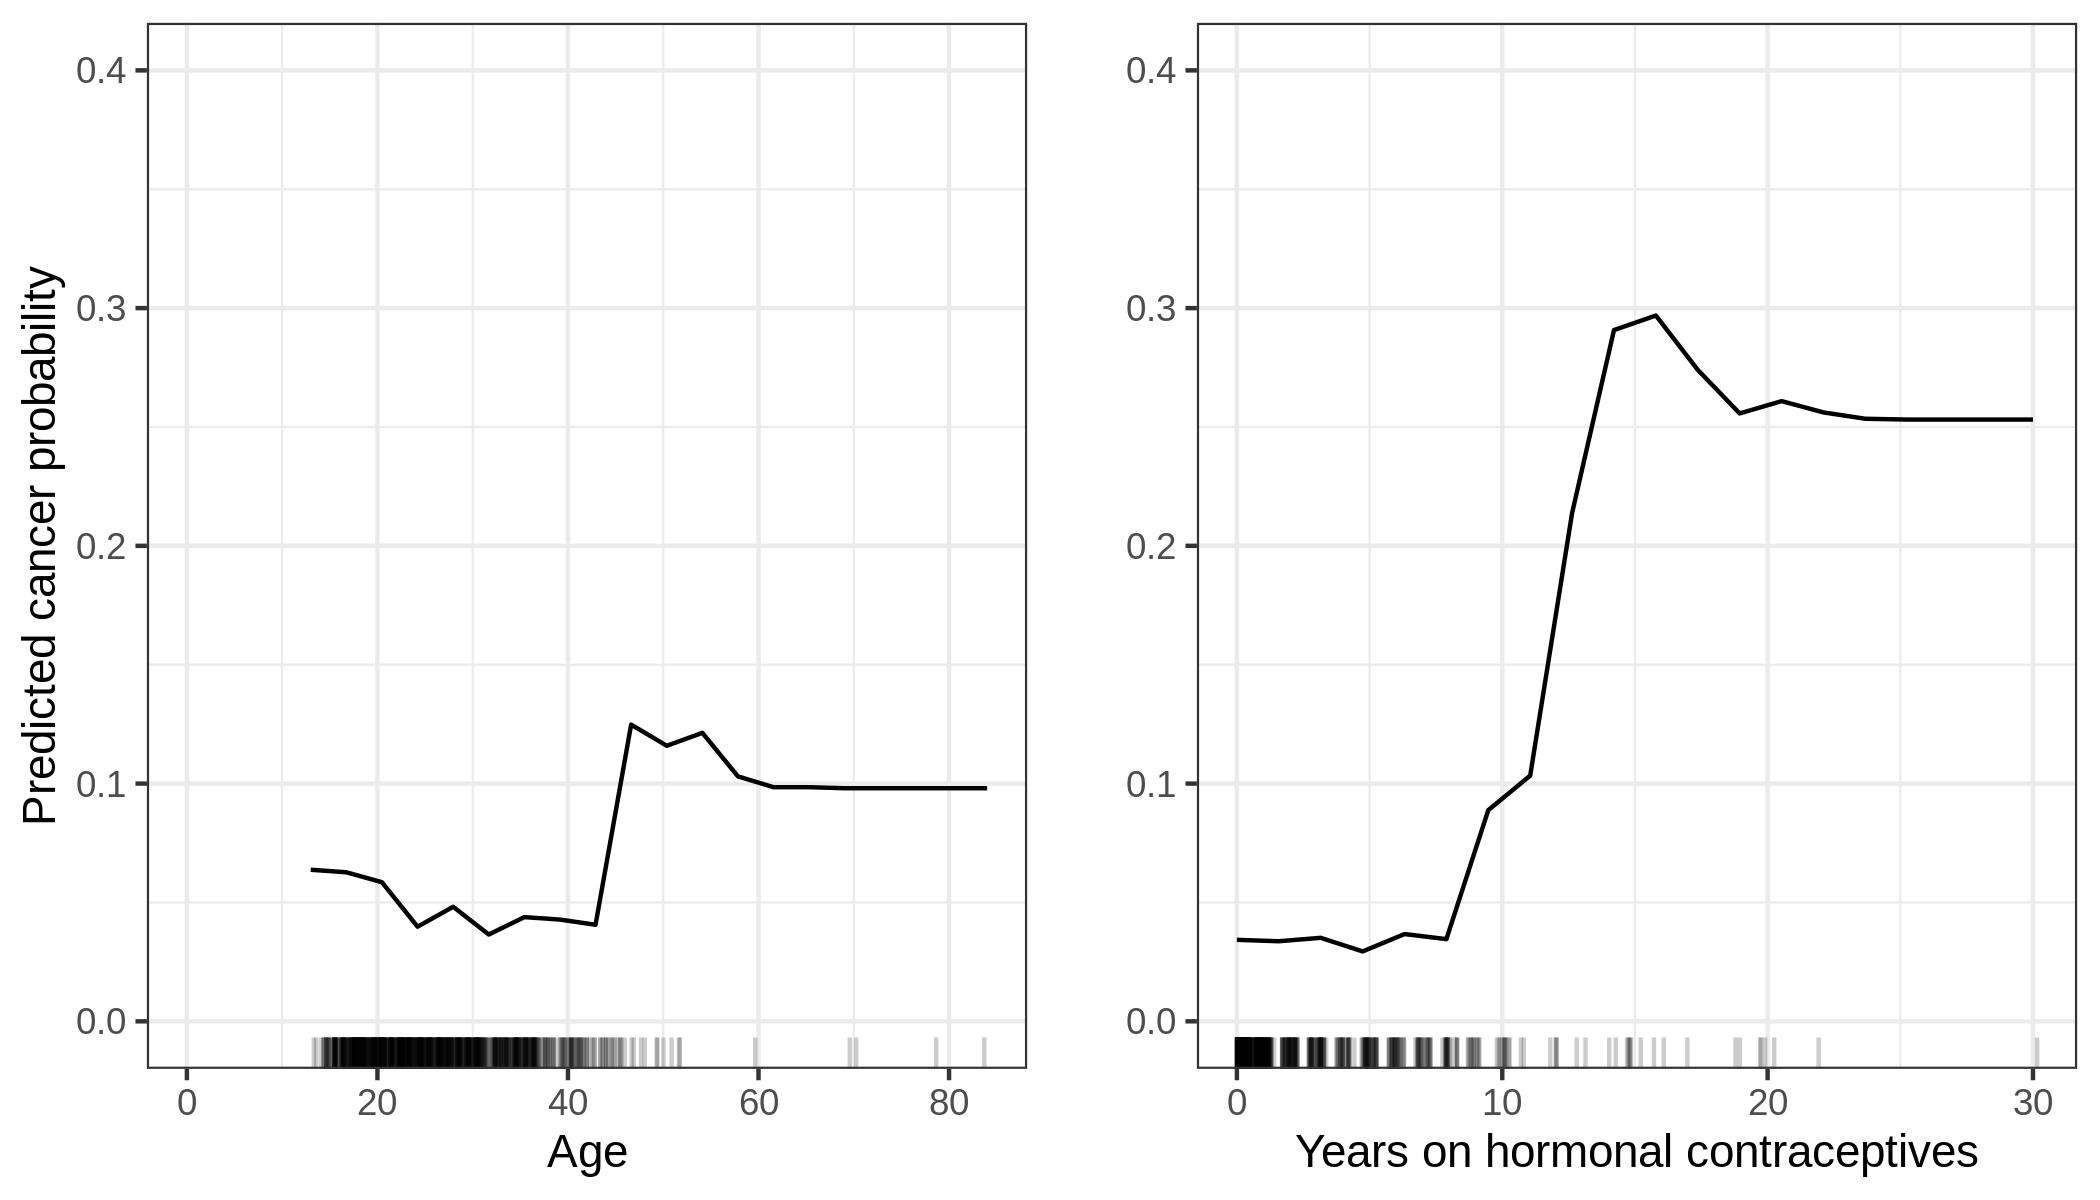
\includegraphics[width=0.7\textwidth]{./figures/pdp-cervical-1.jpeg}
    \caption{Image taken from Interpretable ML book~\citep{molnar2022}}
  \end{figure}

  \noindent\makebox[\linewidth]{\rule{\paperwidth}{0.4pt}}
  Feature Effect is simple and intuitive.
\end{frame}


\begin{frame}
  \frametitle{Feature Effect Methods}
  \begin{itemize}
  \item<1-> PDP
    \begin{itemize}
    \item Expected outcome over \(x_c\): \(f(x_s) = \mathbb{E}_{\mathbf{x_c}}[f(x_s, \mathbf{x_c})]\)
    \item \textbf{Unrealistic instances}
    \end{itemize}

  \item<2-> MPlot
    \begin{itemize}
    \item Expected outcome over \(x_c|x_s\): \(f(x_s) = \mathbb{E}_{\mathbf{x_c}|x_s}[f(x_s, \mathbf{x_c})]\)
    \item \textbf{Aggregated effects}
    \end{itemize}

  \item<3-> ALE
    \begin{itemize}
    \item \(f(x_s) = \int_{x_{min}}^{x_s}\mathbb{E}_{\mathbf{x_c}|x_s=z}[ \frac{\partial f}{\partial x_s}(x_s, \mathbf{x_c})] \partial z\)
    \item \textbf{Resolves both failure modes}
    \end{itemize}

  \end{itemize}
  \noindent\makebox[\linewidth]{\rule{\paperwidth}{0.4pt}}
  PDP vs MPlot vs \alert{ALE}
\end{frame}


\begin{frame}
  \frametitle{ALE approximation}
  ALE definition: \( f(x_s) = \int_{x_{min}}^{x_s}\mathbb{E}_{\mathbf{x_c}|x_s=z}[ \frac{\partial f}{\partial x_s}(x_s, \mathbf{x_c})] \partial z \)
  \noindent\makebox[\linewidth]{\rule{\paperwidth}{0.4pt}}
  ALE approximation from \(\mathcal{D} = { \{\mathbf{x}^i, y^i}\}_{i=1}^N\)

    \[f(x_s) = \sum_k^{k_x} \underbrace{\frac{1}{|\mathcal{S}_k|} \sum_{i:\xb^i \in \mathcal{S}_k} \underbrace{[f(z_k, \mathbf{x^i_c}) - f(z_{k-1}, \mathbf{x^i_c})]}_{\text{point effect}}}_{\text{bin effect}} \]

    \begin{itemize}
    \item Slow \( \rightarrow \) 2 evaluations of \(f\) per point
    \item Restrictive \( \rightarrow\) change bin limits, pay again \(2*N\) evaluations of \(f\)
    \item Insecure \( \rightarrow\) broad bins may create out of distribution samples instances
    \end{itemize}

  \noindent\makebox[\linewidth]{\rule{\paperwidth}{0.4pt}}
  ALE approximation has some disadvantages
\end{frame}




\begin{frame}
  \frametitle{DALE - Differential ALE}
  ALE definition:\(f(x_s) = \Delta x \int_{x_{min}}^{x_s}\mathbb{E}_{\mathbf{x_c}|x_s=z}[ \frac{\partial f}{\partial x_s}(x_s, \mathbf{x_c})] \partial z\)
  \noindent\makebox[\linewidth]{\rule{\paperwidth}{0.4pt}}
  DALE, from the dataset \(\mathcal{D} = { \{\mathbf{x}^i, y^i}\}_{i=1}^N\)

    \[f(x_s) = \sum_k^{k_x} \underbrace{\frac{1}{|\mathcal{S}_k|} \sum_{i:\xb^i \in \mathcal{S}_k} \underbrace{[\frac{\partial f}{\partial x_s}(x_s^i, \mathbf{x^i_c})]}_{\text{point effect}}}_{\text{bin effect}} \]

    \begin{itemize}
    \item Fast \( \rightarrow \) use of auto-differentiation, all derivatives in a single pass
    \item Versatile \( \rightarrow\) point effects computed once, change bins without cost
    \item Secure \( \rightarrow\) does not create artificial instances
    \end{itemize}

  \noindent\makebox[\linewidth]{\rule{\paperwidth}{0.4pt}}
  DALE is a better approximation of ALE, for \alert{differentiable} models
\end{frame}



% chapter 1
\section{DALE vs ALE}

\subsection{Dale is faster and versatile}

\begin{frame}
  \frametitle{DALE is faster and versatile - Theory}
    \[f(x_s) = \sum_k^{k_x} \underbrace{\frac{1}{|\mathcal{S}_k|} \sum_{i:\xb^i \in \mathcal{S}_k} \underbrace{[\frac{\partial f}{\partial x_s}(x_s^i, \mathbf{x^i_c})]}_{\text{point effect}}}_{\text{bin effect}} \]

  \begin{itemize}
  \item Faster
    \begin{itemize}
      \item gradients wrt all features \(\nabla_{\mathbf{x}} f(\mathbf{x^i})\) in a single pass
      \item auto-differentiation must be available (deep learning)
    \end{itemize}
  \item Versatile
    \begin{itemize}
    \item Change bin limits, with near zero computational cost
    \end{itemize}

  \end{itemize}
  \noindent\makebox[\linewidth]{\rule{\paperwidth}{0.4pt}}
  DALE is faster and allows redefining bin-limits
\end{frame}

\begin{frame}
  \frametitle{DALE is faster and versatile - Experiments}
  \begin{figure}[h]
  \centering
  \resizebox{.4\columnwidth}{!}{% This file was created with tikzplotlib v0.10.1.
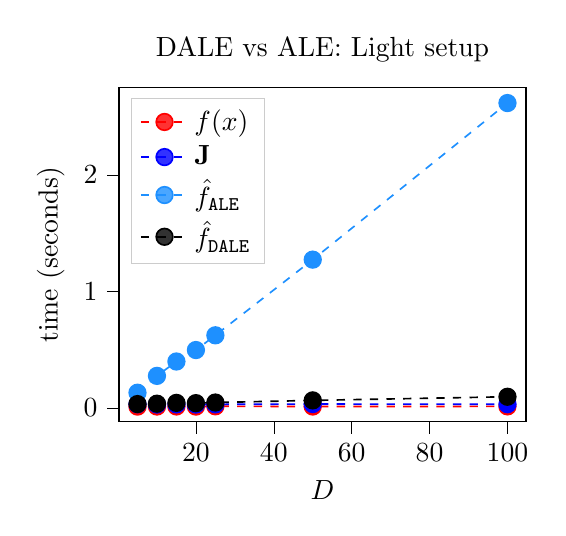
\begin{tikzpicture}

\definecolor{darkgray176}{RGB}{176,176,176}
\definecolor{dodgerblue}{RGB}{30,144,255}
\definecolor{lightgray204}{RGB}{204,204,204}

\begin{axis}[
legend cell align={left},
legend style={
  fill opacity=0.8,
  draw opacity=1,
  text opacity=1,
  at={(0.03,0.97)},
  anchor=north west,
  draw=lightgray204
},
tick align=outside,
tick pos=left,
title={DALE vs ALE: Light setup},
x grid style={darkgray176},
xlabel={\(\displaystyle D\)},
xmin=0.25, xmax=104.75,
xtick style={color=black},
y grid style={darkgray176},
ylabel={time (seconds)},
ymin=-0.118335867500491, ymax=2.74596303149951,
ytick style={color=black}
]
\addplot [semithick, red, dashed, mark=*, mark size=3, mark options={solid}]
table {%
5 0.0118595361709595
10 0.0122641324996948
15 0.0128312110900879
20 0.0119729042053223
25 0.0144194364547729
50 0.0124425888061523
100 0.0135363340377808
};
\addlegendentry{$f(x)$}
\addplot [semithick, blue, dashed, mark=*, mark size=3, mark options={solid}]
table {%
5 0.0321429967880249
10 0.0295344591140747
15 0.0305428504943848
20 0.0298470258712769
25 0.0309284925460815
50 0.0336670875549316
100 0.032146692276001
};
\addlegendentry{$\mathbf{J}$}
\addplot [semithick, dodgerblue, dashed, mark=*, mark size=3, mark options={solid}]
table {%
5 0.130752086639404
10 0.275371313095093
15 0.398597836494446
20 0.496960043907166
25 0.623412370681763
50 1.27240407466888
100 2.61576771736145
};
\addlegendentry{$\hat{f}_{\mathtt{ALE}}$}
\addplot [semithick, black, dashed, mark=*, mark size=3, mark options={solid}]
table {%
5 0.0335890054702759
10 0.0366946458816528
15 0.0436010360717773
20 0.0414165258407593
25 0.0466822385787964
50 0.0650126934051514
100 0.0961912870407104
};
\addlegendentry{$\hat{f}_{\mathtt{DALE}}$}
\end{axis}

\end{tikzpicture}
}
  \resizebox{.43\columnwidth}{!}{% This file was created with tikzplotlib v0.10.1.
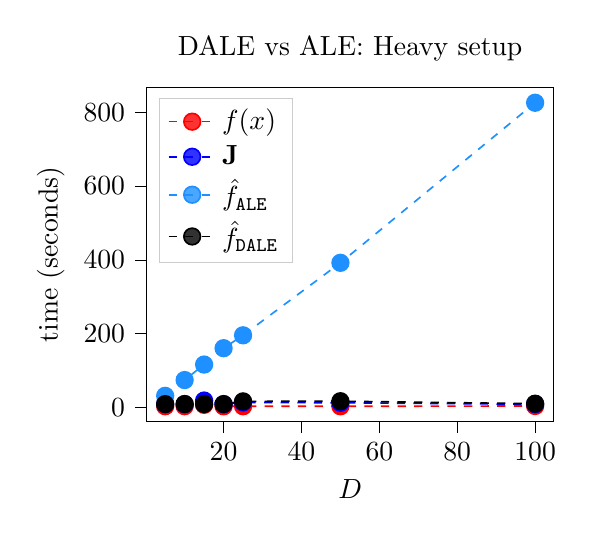
\begin{tikzpicture}

\definecolor{darkgray176}{RGB}{176,176,176}
\definecolor{dodgerblue}{RGB}{30,144,255}
\definecolor{lightgray204}{RGB}{204,204,204}

\begin{axis}[
legend cell align={left},
legend style={
  fill opacity=0.8,
  draw opacity=1,
  text opacity=1,
  at={(0.03,0.97)},
  anchor=north west,
  draw=lightgray204
},
tick align=outside,
tick pos=left,
title={DALE vs ALE: Heavy setup},
x grid style={darkgray176},
xlabel={\(\displaystyle D\)},
xmin=0.25, xmax=104.75,
xtick style={color=black},
y grid style={darkgray176},
ylabel={time (seconds)},
ymin=-38.1810145603003, ymax=867.056094992299,
ytick style={color=black}
]
\addplot [semithick, red, dashed, mark=*, mark size=3, mark options={solid}]
table {%
5 3.13364505767822
10 3.24496150016785
15 6.86045789718628
20 2.96612668037415
25 3.05197858810425
50 3.02510833740234
100 3.71672296524048
};
\addlegendentry{$f(x)$}
\addplot [semithick, blue, dashed, mark=*, mark size=3, mark options={solid}]
table {%
5 8.88222980499268
10 8.82908821105957
15 18.4925575256348
20 8.51719951629639
25 13.5228071212769
50 12.4858655929565
100 8.59451198577881
};
\addlegendentry{$\mathbf{J}$}
\addplot [semithick, dodgerblue, dashed, mark=*, mark size=3, mark options={solid}]
table {%
5 31.310697555542
10 74.1438674926758
15 116.133689880371
20 160.465118408203
25 195.409912109375
50 391.950622558594
100 825.908935546875
};
\addlegendentry{$\hat{f}_{\mathtt{ALE}}$}
\addplot [semithick, black, dashed, mark=*, mark size=3, mark options={solid}]
table {%
5 8.83595371246338
10 9.03882694244385
15 9.21370220184326
20 8.9499044418335
25 16.3313121795654
50 16.7110271453857
100 10.0340776443481
};
\addlegendentry{$\hat{f}_{\mathtt{DALE}}$}
\end{axis}

\end{tikzpicture}
}
  \caption[Case-1-fig-1]{Light setup; small dataset, light \(f\). Heavy setup; big dataset (\(N=10^5\)), heavy \(f\)}
  \label{fig:case-1-plots-1}
\end{figure}

  \noindent\makebox[\linewidth]{\rule{\paperwidth}{0.4pt}}
  DALE considerably accelerates the estimation
\end{frame}


\subsection{DALE is more Accurate}

\begin{frame}
  \frametitle{DALE uses only on-distribution samples}
    \[f(x_s) = \sum_k^{k_x} \underbrace{\frac{1}{|\mathcal{S}_k|} \sum_{i:\xb^i \in \mathcal{S}_k} \underbrace{[\frac{\partial f}{\partial x_s}(x_s^i, \mathbf{x^i_c})]}_{\text{point effect}}}_{\text{bin effect}} \]

  \begin{itemize}
  \item Faster
    \begin{itemize}
      \item gradients wrt all features \(\nabla_{\mathbf{x}} f(\mathbf{x^i})\) in a single pass
      \item auto-differentiation must be available (deep learning)
    \end{itemize}
  \item Versatile
    \begin{itemize}
    \item Change bin limits, with near zero computational cost
    \end{itemize}

  \end{itemize}
  \noindent\makebox[\linewidth]{\rule{\paperwidth}{0.4pt}}
  DALE is faster and allows redefining bin-limits
\end{frame}

\begin{frame}
  \frametitle{DALE vs ALE - 3 Bins}
  \begin{figure}[ht]
    \centering
    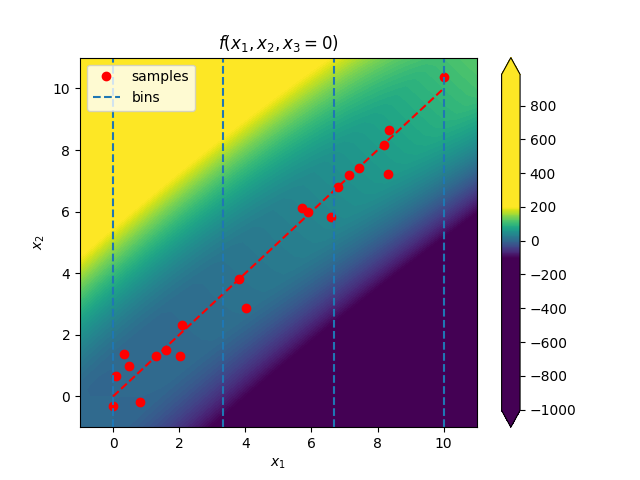
\includegraphics[width=0.4\textwidth]{./figures/bin_splitting_3_bins.png}\\
    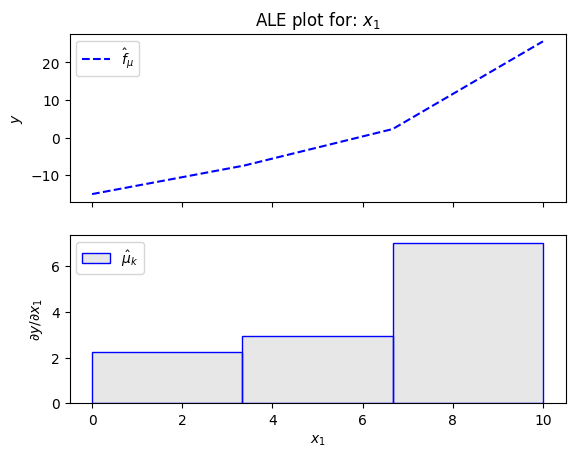
\includegraphics[width=0.4\textwidth]{./figures/dale_3_bins.png}
    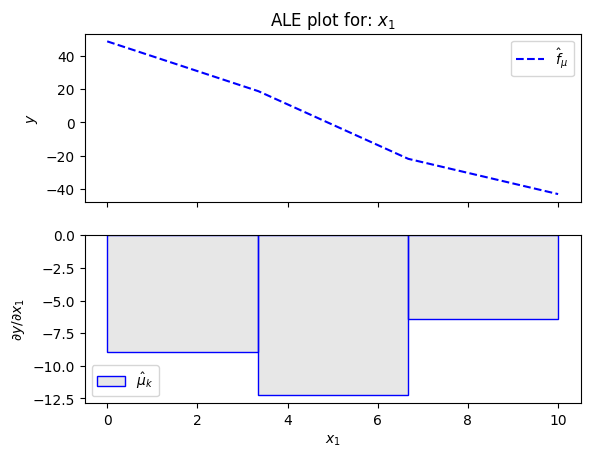
\includegraphics[width=0.4\textwidth]{./figures/ale_3_bins.png}
    \label{}
  \end{figure}
  \noindent\makebox[\linewidth]{\rule{\paperwidth}{0.4pt}}
  We search for a \alert{single configuration (point-estimate) \( \hat{\thetab}\) }
\end{frame}



\begin{frame}
  \frametitle{DALE vs ALE - 5 Bins}
  \begin{figure}[ht]
    \centering
    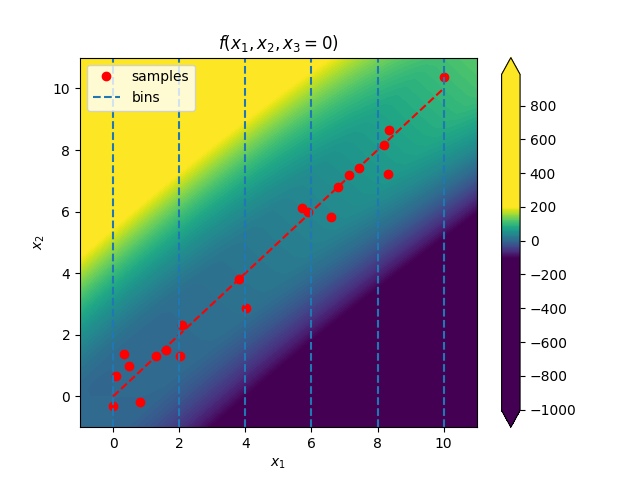
\includegraphics[width=0.4\textwidth]{./figures/bin_splitting_5_bins.png}\\
    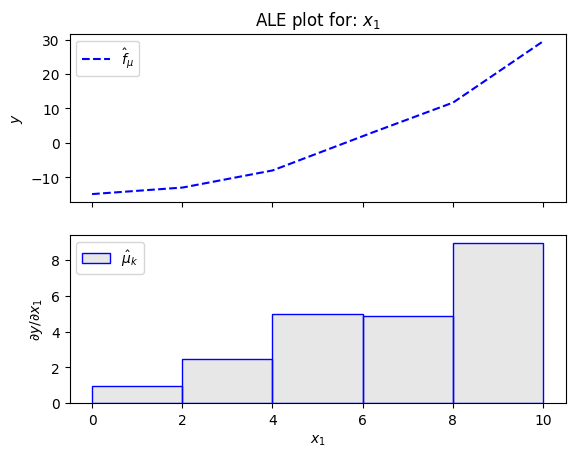
\includegraphics[width=0.4\textwidth]{./figures/dale_5_bins.png}
    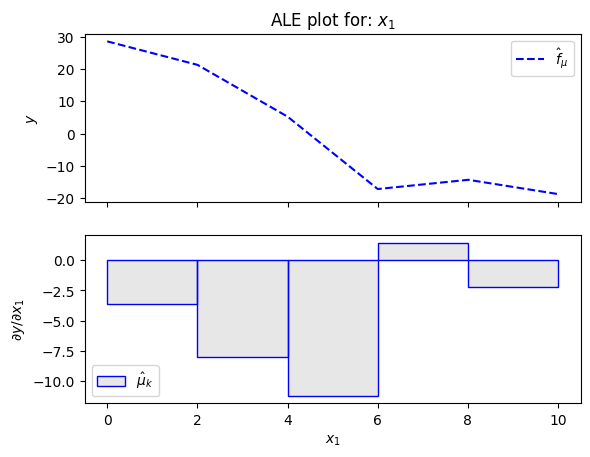
\includegraphics[width=0.4\textwidth]{./figures/ale_5_bins.png}
    \label{}
  \end{figure}
  \noindent\makebox[\linewidth]{\rule{\paperwidth}{0.4pt}}
  We search for a \alert{single configuration (point-estimate) \( \hat{\thetab}\) }
\end{frame}


\begin{frame}
  \frametitle{DALE vs ALE - 10 Bins}
  \begin{figure}[ht]
    \centering
    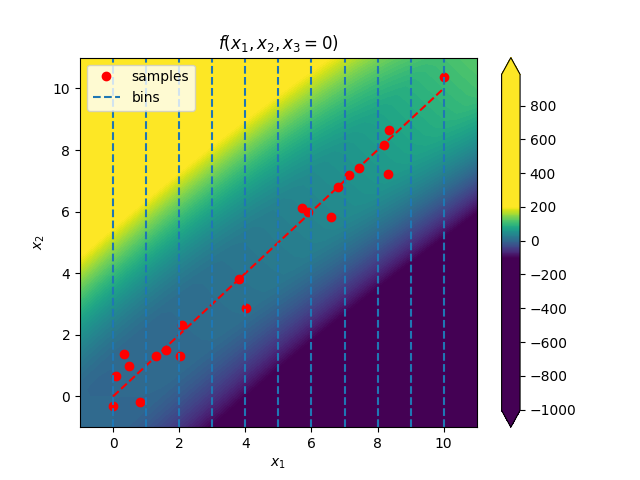
\includegraphics[width=0.4\textwidth]{./figures/bin_splitting_10_bins.png}\\
    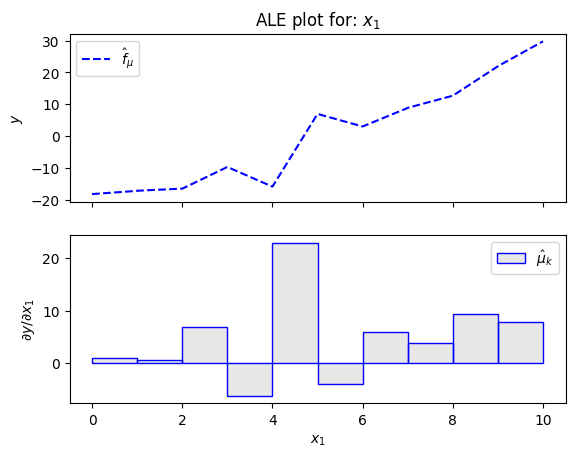
\includegraphics[width=0.4\textwidth]{./figures/dale_10_bins.png}
    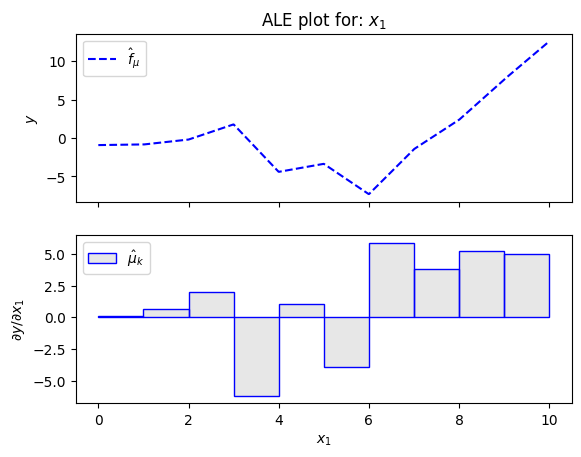
\includegraphics[width=0.4\textwidth]{./figures/ale_10_bins.png}
    \label{}
  \end{figure}
  \noindent\makebox[\linewidth]{\rule{\paperwidth}{0.4pt}}
  We search for a \alert{single configuration (point-estimate) \( \hat{\thetab}\) }
\end{frame}


\begin{frame}
  \frametitle{DALE vs ALE - 20 Bins}
  \begin{figure}[ht]
    \centering
    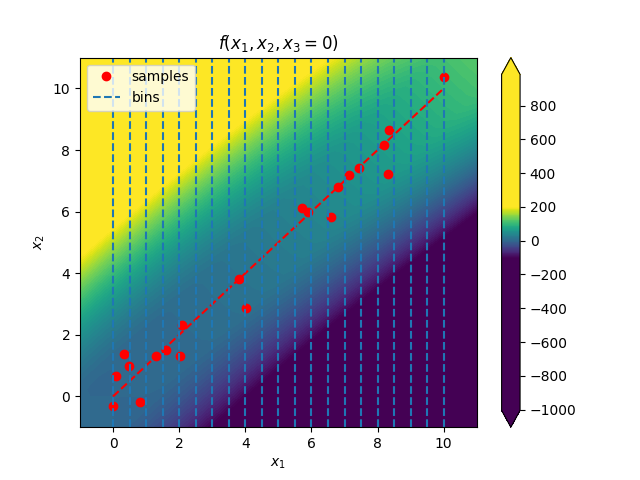
\includegraphics[width=0.4\textwidth]{./figures/bin_splitting_20_bins.png}\\
    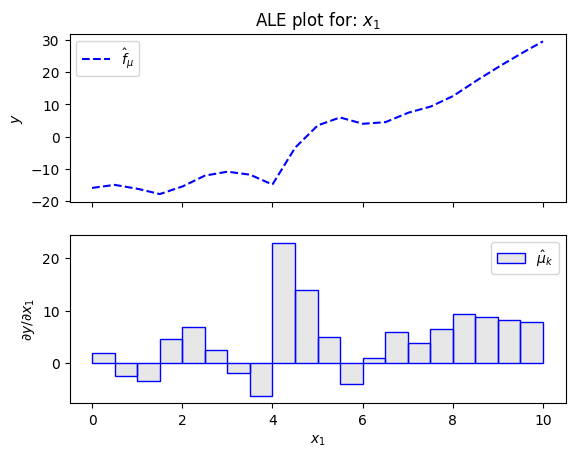
\includegraphics[width=0.4\textwidth]{./figures/dale_20_bins.png}
    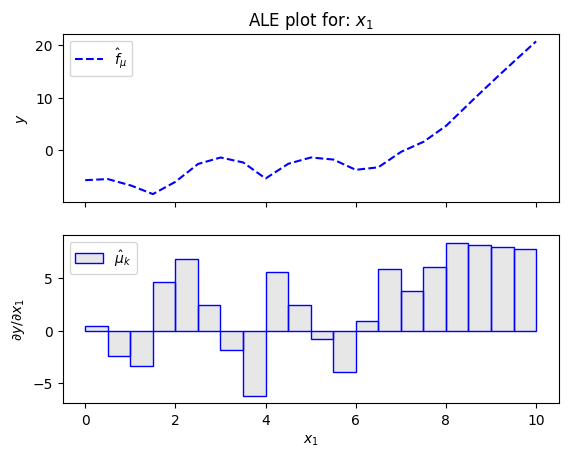
\includegraphics[width=0.4\textwidth]{./figures/ale_20_bins.png}
    \label{}
  \end{figure}
  \noindent\makebox[\linewidth]{\rule{\paperwidth}{0.4pt}}
  We search for a \alert{single configuration (point-estimate) \( \hat{\thetab}\) }
\end{frame}


\begin{frame}
  \frametitle{DALE vs ALE - 40 Bins}
  \begin{figure}[ht]
    \centering
    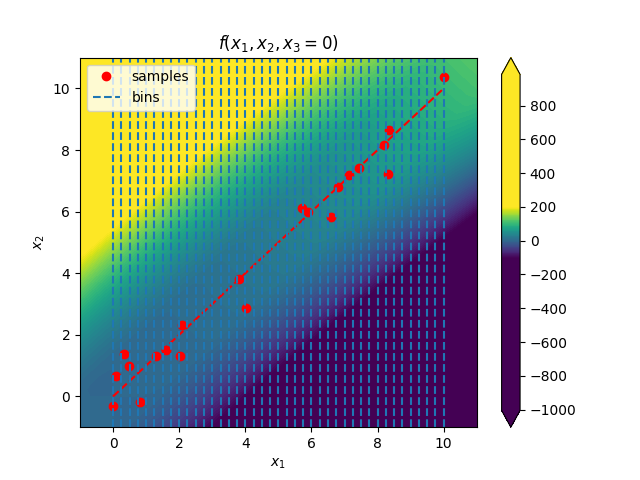
\includegraphics[width=0.4\textwidth]{./figures/bin_splitting_40_bins.png}\\
    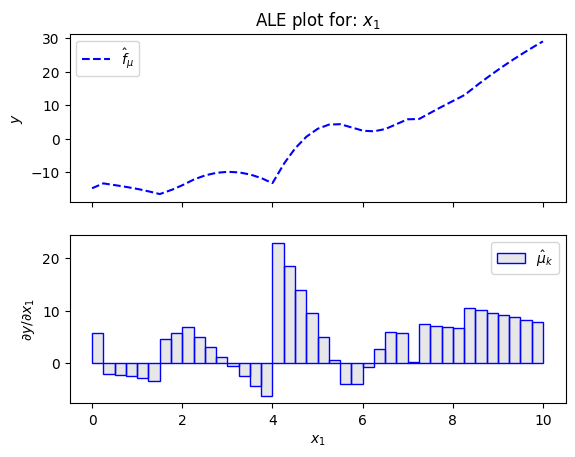
\includegraphics[width=0.4\textwidth]{./figures/dale_40_bins.png}
    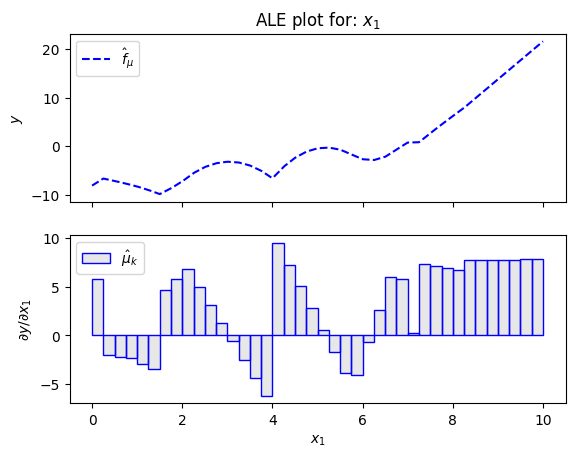
\includegraphics[width=0.4\textwidth]{./figures/ale_40_bins.png}
    \label{}
  \end{figure}
  \noindent\makebox[\linewidth]{\rule{\paperwidth}{0.4pt}}
  We search for a \alert{single configuration (point-estimate) \( \hat{\thetab}\) }
\end{frame}

\section{Future Work}

\begin{frame}
  \frametitle{What next?}
  \begin{figure}[ht]
    \centering
    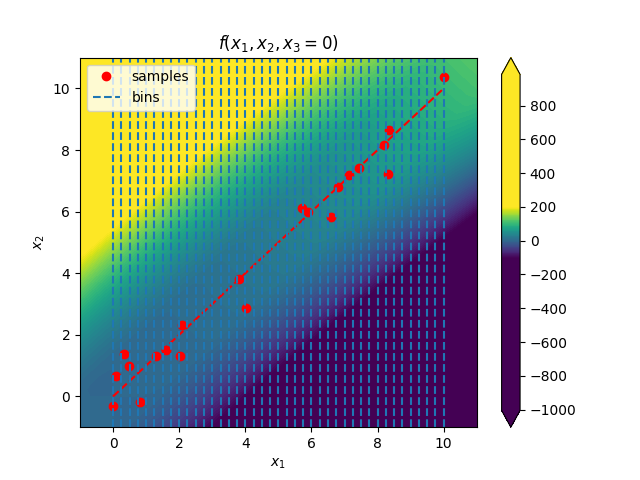
\includegraphics[width=0.4\textwidth]{./figures/bin_splitting_40_bins.png}\\
    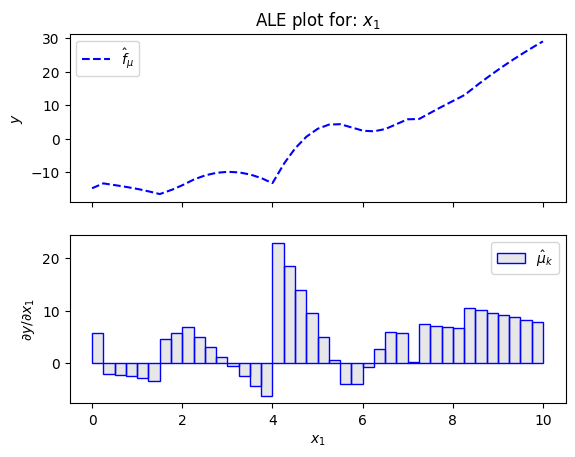
\includegraphics[width=0.4\textwidth]{./figures/dale_40_bins.png}
    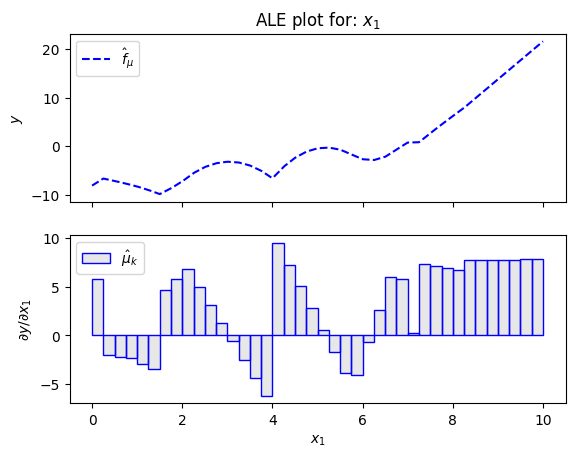
\includegraphics[width=0.4\textwidth]{./figures/ale_40_bins.png}
    \label{}
  \end{figure}
  \noindent\makebox[\linewidth]{\rule{\paperwidth}{0.4pt}}
  DALE advantages can be a driver for future work
\end{frame}





\begin{frame}[allowframebreaks]
  \frametitle{References}
  \bibliography{bibliography.bib}
\end{frame}


\end{document}